\documentclass[landscape,twocolumn]{article}
\usepackage{biblatex, graphicx, hyperref, mathtools, pgfplots, pgfplotstable}
\addbibresource{references.bib}
\pgfplotsset{compat = 1.16}
\title{COMP5318 Assignment 1}
\author{Nicholas Grasevski (ngra5777, 500710654)}
\begin{document}
\maketitle
\begin{abstract}
	In this report several image classifiers are benchmarked against a grayscale image dataset. With the help of some feature engineering, a linear Support Vector Machine is the highest performing classifier with 89.65\% accuracy on the test set.
\end{abstract}

\section{Introduction}
Object recognition is one of the biggest subfields of computer vision, with many practical applications such as computer aided diagnosis~\cite{doi2007computer}, face detection~\cite{hjelmaas2001face}, Optical Character Recognition~\cite{mori1999optical} and so on.

The current state of the art in object recognition is Convolutional Neural Networks~\cite{iandola2016squeezenet}. The convolutional neural network takes in the raw pixel data and applies several layers of `convolution' transformations, which aggregate nearby pixels into higher order features in a hierarchical fashion. Prior to the prevalence of GPU based neural network training, the previous state of the art was to apply some hand crafted transformations to the input image to extract higher order features~\cite{rybski2010visual}, and then pass the encoded features through a classical machine learning algorithm such as a generalized linear model~\cite{ebrahimzadeh2014efficient}.

The aim of this study is to compare and contrast several different machine learning algorithms when applied to an object detection problem. This should provide insight into their relative ability to capture the information in the data, with the help of some standard hand crafted feature transformations.

\section{Methods}
Describe the pre-processing techniques and classifier methods algorithms.

\begin{figure}[ht]
	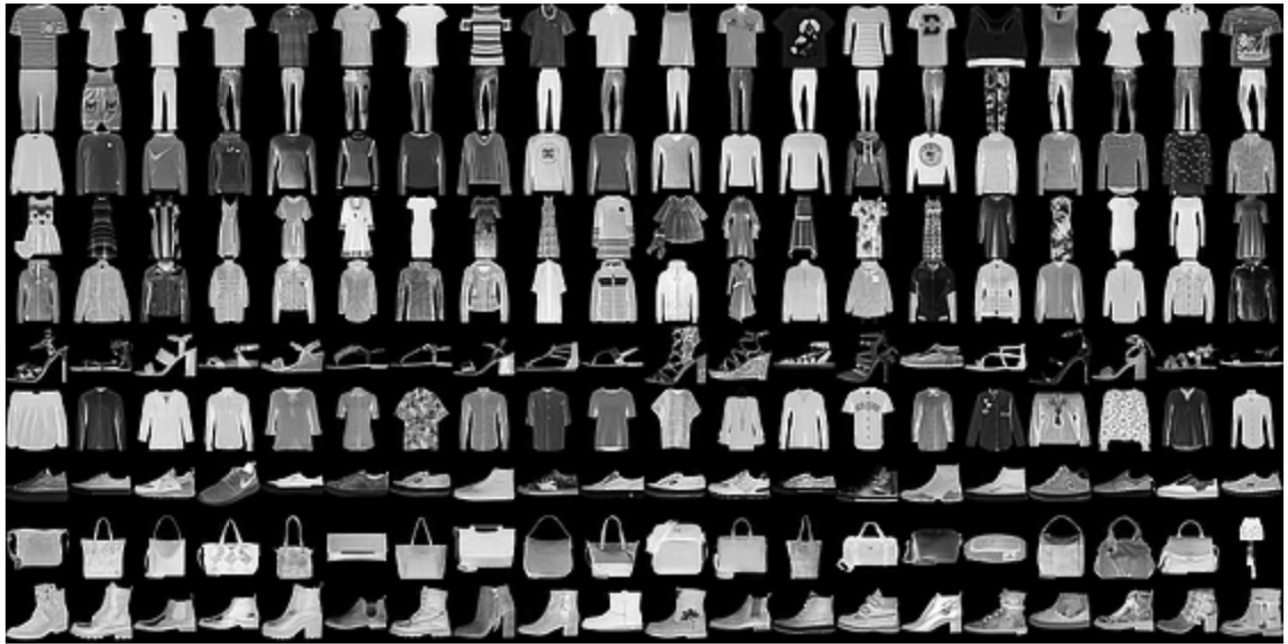
\includegraphics[width=\linewidth]{../Dataset_image}
	\caption{Grayscale $28 \times 28$ images of clothing.}\label{fig:images}
\end{figure}

Several machine learning algorithms were benchmarked against a corpus of $28 \times 28$ grayscale images. Examples of the images can bee seen in figure~\ref{fig:images}. There are 10 classes in total:
\begin{enumerate}
	\item T-shirt/Top
	\item Trouser
	\item Pullover
	\item Dress
	\item Coat
	\item Sandal
	\item Shirt
	\item Sneaker
	\item Bag
	\item Ankle Boot
\end{enumerate}

30,000 of these images are used for training and hyperparameter tuning using 10-fold cross-validation, and 2,000 are used as a hold-out set to evaluate the best classifier according to the hyperparameter tuning results.

The performance is evaluated primarily based on top-1 accuracy, as defined in equation~\ref{eq:accuracy}:

\begin{equation}
	\label{eq:accuracy}
	\text{Accuracy} = \frac{\text{Number of correct classifications}}{\text{Total number of test examples used}}
\end{equation}

The training and inference time cost of each algorithm is also evaluated. The experiment was performed on a 16-inch 2019 MackBook Pro, with a 2.3GHz 8-Core Intel Core i9 and 32 GB 2667 MHz DDR4 RAM\@.

\subsection{Preprocessing}
\begin{figure}[ht]
	\includegraphics[width=\linewidth]{../Output/hog}
	\caption{Histogram of Oriented Gradients transformation.}\label{fig:hog}
\end{figure}

The input data was preprocessed using a feature descriptor called `Histogram of Oriented Gradients' (HOG)~\cite{dalal2005histograms}. It performs the following steps:
\begin{description}
	\item[Gamma compression] First, the square root of the raw pixel data is taken to reduce the influence of illumination effects.
	\item[Gradient computation] The horizontal and vertical gradients between adjacent pixels are calculated, resulting in each cell having a 2D gradient vector.
	\item[Orientation binning] The orientations of these vectors are discretized, into 9 bins in our case, corresponding to bins from 0 to 180 degrees.
	\item[Cell histogram] These discretized orientations are then aggregated by `cells', which in our case are $7 \times 7$ pixel areas, and collected in a histogram, with each pixel orientation contributing to the histogram according to its magnitude.
	\item[Descriptor blocks] The cells are then grouped into `blocks', which in our case are $2 \times 2$ pixel areas, in a sliding window fashion.
	\item[Block normalization] The cells in each block are normalized against one another using the $L_1$ norm in our case.
	\item[Object detection] Finally, the overlapping normalized blocks are flattened into a feature vector, to be fed into a machine learning algorithm.
\end{description}

The HOG descriptor achieves the following tasks:

\begin{description}
	\item[Normalization] The block descriptor normalization provides better invariance to illumination, shadowing, and edge contrast.
	\item[Dimensionality Reduction] The histogram grouping effectively downscales the image data, reducing the original length-784 feature vector ($28 \times 28$) down to 324 ($\text{9 orientations} \times \text{4 cells per block} \times \text{9 blocks}$). This speeds up training, makes it more robust and reduces variance, at the cost of some loss of information and thus an increase in bias.
	\item[Feature Extraction] The raw pixel data is distilled to a more meaningful representation of the object edges, as can be seen in figure~\ref{fig:hog}.
\end{description}

\subsection{Algorithms}
Several different algorithms are applied in turn to the preprocessed data, and a grid of their hyperparameters are explored. A stratified 10-fold cross validation is performed on each hyperparameter combination and the highest scoring (algorithm, hyperparameter) combination is retrained on the entire training set and evaluated on the test set.

% TODO

\subsubsection{Nearest Neighbor}
\subsubsection{Logistic Regression}
\subsubsection{Naive Bayes}
\subsubsection{Decision Tree}
\subsubsection{Bagging}
\subsubsection{Ada Boost}
\subsubsection{Support Vector Machine}

\section{Experiments and results}
% TODO
Comparing experiment results between different algorithms (using table or graph) and produce a meaningful discussion of results from the experiment and choice of classifier methods (analysis on potential reasons for good performance or bad performance, and for training and inference time consumption).

\section{Conclusion}
Out of the algorithms applied, Support Vector Machine achieved the highest accuracy at the expense of a relatively long training time. Naive Bayes was by far the fastest in both training and inference, due to the efficient time complexity of the algorithm. Further improvements would be to consider convolutional neural networks in order to automatically extract similar features to the HOG descriptor via backpropagation and stochastic gradient descent. Furthermore, GPU acceleration could be utilized to achieve fast training and inference by parallelizing the pixel-wise operations which are very common in computer vision.

\printbibliography\appendix
\section{Running the code}
\begin{description}
	\item[Dependencies] \texttt{pip3 install h5py pandas scikit-image scikit-learn}
	\item[Usage] Run the steps in the notebook sequentially to get the tuning and evaluation results.
\end{description}

Detailed hyperparameter tuning results will be written as csv files to \texttt{Output} for each respective classifier, along with the final predictions as \texttt{Output/predicted\_labels.h5}. Note that the \texttt{ALGORITHMS} parameter can be modified at will to change the grid search process, for example to speed up the runtime of the script by excluding certain algorithms or hyperparameter combinations.

\end{document}
